\documentclass[a4paper,11pt]{article}
\usepackage{amssymb}
\usepackage{booktabs}
\usepackage{geometry}
%\usepackage[hidelinks]{hyperref}
\usepackage{listings}
%\usepackage{lipsum}
\usepackage{graphicx}
\usepackage{natbib}

\bibliographystyle{plain}

\geometry{
	includeheadfoot,
	margin=2.54cm
}

\title{
	2IV55 Interactive Virtual Environments: Final Report \\
	\small{Group 2}
}
\author{
	Tim van Dalen (0744839)
	\and
	Robbert Jongeling (0747896)
	\and
	Jasper Selman (0741516)
	\and
	Ramon de Vaan (0758873)
	\and
	Bart van Wezel (0740608)
}
\date{\today}

\begin{document}
	\maketitle
	
	\begin{abstract}
	$<$abstract$>$
	\end{abstract}
		
	\section{Introduction}
\subsection{Context}\label{sec:context}
Virtual worlds are getting more and more realistic and there are getting more techniques to visualize these worlds in 3D. One of those techniques are head mounted displays. Head mounted displays are more and more common. Most people can make one themself with a cardboard and two lenses. Head mounted devices are quickly becoming more advanced and realistic. The resolution gets better and there getting more applications that make great use of the benefits of head mounted devices. 
\subsection{Problem Definition}\label{sec:problem}
However interacting with these world while wearing a head mounted display remains a problem. Especially moving around is a difficult problem, because with increasing sizes of the virtual world, the user would need a very large empty room. This is surely not possible for everyone and thus solutions are needed for this problem. 
Our research is about ``redirected walking", a technique to let users walk through a large virtual environment using a head mounted display. ``Redirected walking"  applies different rotational gains and translation gains without the user noticing. 
``Rotational gains cause a user's rate of rotation in virtual space to by either greater or less than 
the user's physical rotation. This can be applied when the user rotates his head or upper body 
without moving his legs, or when the user rotates by adjusting his footing. For example, if the 
user rotates 60 degrees in the real world, a rotational gain of 5/4 could be applied so that the 
user rotates 75 degrees in the virtual world."\cite{jwalker}
Translation gains cause a user's translation in the virtual space to be greater or less than the actual translation. Thus if the user walks 2 meter in the real world, this could be 1.5 meter or 2.5 meter in the virtual world. \\
We focus our research on rotational gains, because we only have limited time for this project. We chose for the rotatinal gains, because the translation in the real world are hard to measure.

\subsection{Research questions}\label{sec:questions}
Our research question is: At what rotational gains does the user notice that the virtual world and the real world rotations are different? And is this number different when a user is engaged in a task versus when a user is just walking around without specific task? (other than walking around).

\subsection{Approach}\label{sec:approach}
We wanted to find the answers to these questions by letting two groups walk through a virtual environment with different rotational gains. We need to bind the movements of the virtual world to the movements that the subjects make in real life.
This will most likely require us to program using an Oculus Rift SDK, with the added possibility for us to change the rotation ratio, i.e. the amount of real world rotation in comparison with the amount of virtual world rotation.
A test subject will attempt to follow a path, with a given rotation ratio.
Some users (about half of our test group) will be asked to conduct a task while following a path, such as counting a number of objects in the world. The other users will only walk the path. At the end of the path, the user is asked to point towards his starting position, this will give us an indication of the perceived rotation. Then, the user is asked whether he has noticed anything, this will indicate whether he has noticed any difference in rotation between the virtual and the real world at all. Finally, we will ask the user to indicate whether he thinks the actual rotation is greater, equal or smaller than the virtual rotation.

\subsection{Introduction}\label{sec:intro}
We will first discuss all the work that is related to our problem and research question. Here we will discuss some virtual realtiy concepts that are important for our experiment. We will also tell something about the Oculus Rift DK2, because it is an important part of our exerpiment. After that we will discuss all the related  research to redirected walking. \\
Then we will describe how we conducted the experiment. How our experiment relates to the research questions and  what bottlenecks we encountered during the experiment design and the eventual experiment. \\
After that we will describe what the results of how experiment where and discuss these results. We will describe what we learned from this experiment and show how the results relate to the results of related work. \label{sec:intro}
	%set the context, what is the problem?, what are the questions?, what is the approach ?

	\section{Related work}
We now discuss virtual reality concepts and research in the field of virtual reality related to our experiment.
First virtual reality concepts, in particular, concepts related to \textit{presence}.
Then related research, in particular focussing on redirected walking techniques.

\subsection{Virtual Reality Concepts}\label{sec:concepts}
The Oculus Rift is a head mounted display and uses an \textit{egocentric} viewpoint. 
I.e., the perceived viewpoint and orientation are that of the self.
This in contrast to an \textit{exocentric} viewpoint, in which the viewpoint is a different viewpoint than the self.
Exocentric viewpoints can be found in e.g. third person video games, where the view includes an image of the self.
Naturally, in redirected walking research, we are interested in egocentric viewpoints as we want to investigate the behaviour of test subjects as if they are in the real world.

A virtual reality is said to be \textit{immersive} if the participant has lost awareness of her presence in the real world and it has been replaced by a sense of presence in a virtual world. 
This virtual world then should fully enclose the participant.
Full immersion is achieved when the participant fully believes she is in the virtual world and not in the real world.
We say, the participant feels present.

The VR-concept called \textit{presence} is very important for our experiment.
Presence is defined as ``A mental state in which a user feels physically present within the computer-mediated environment.''
Using the head tracking functionalities of Oculus Rift, we can update the image in real time such that the participant believes she is physically present within the virtual world.
In our experiment, we are interested in finding out when participants lose their sense of presence in the virtual world. 
For this, we need that they initially do feel present to at least some extent.
There are several factors that can contribute to a higher feeling of presence such as the degree of which the the virtual world is realistic.

Another important factor in the feeling of presence is latency of the screen updates with respect to movements of the head.
Ideally, we would like to update the image in real-time, just as in the real world. 
This is not achievable in a HMD such as the Oculus. 
Research has been done to find out the effects of latency on the feeling of presence.\cite{meehan}
This research has shown that higher latency has adverse effects on the feeling of presence.
The Oculus DK2 positional tracker has low latency, it updates with a 60Hz rate.

Using \textit{Substitution} of real data by computer generated data we try to get the participants to walk a different path than what they think. 
The rotational degree of test subjects making a turn can be exaggerated in the virtual world resulting in subjects walking in a tighter curve in reality than in the virtual world.
This influences the feeling of presence, the question is what the threshold is for the user noticing this difference between the virtual and the real world. 
It is likely that for very large differences between the physical world and the virtual world, test subjects will no longer accept the virtual world as real.
They will no longer feel present. 


\subsection{Oculus Rift DK2}
The Oculus Rift DK2 claims to provide ``truly immersive virtual reality" and has a 100 degrees field of view providing a stereoscopic 3D perspective.\cite{oculus}
Head tracking has six degrees of freedom, meaning a user can rotate his head in any possible direction and the view will update in that direction.
Furthermore latency of these updates is low with 60Hz update rate for the positional tracker.
The resolution of the two screens (one per eye) are 960x1080 pixels.
The screen refresh rates are at most 75Hz.
A stock photograph of the DK2 HMD and the positional tracker is included in Figure \ref{fig:dk2}.

\begin{figure}
	\centering
	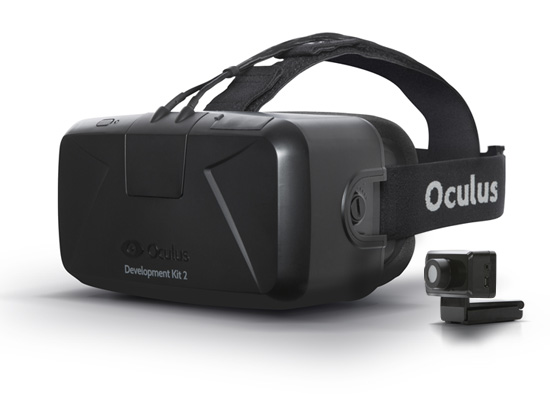
\includegraphics[width=0.5\linewidth]{sections/finalreport/images/dk2.png}	
	\caption{Oculus Rift Development Kit 2 head-mounted display and positional tracker.}
	\label{fig:dk2}
\end{figure}

\subsection{Related  research}
The technique of redirected walking was first introduced by Razzaque et al. in \cite{razzaque}. 
In redirected walking, there are several concepts we can investigate.
There is rotational, translational and curvature redirection.
In addition to these three methods, experiments have been done with dynamic redirection factors.\cite{neth}
In curvature redirection, the virtual world is rotated slightly as the test subject walks forward.
The test subject will then try to correct this rotation which results in him walking on a curved path in the real world while walking on a straight path in the virtual world.
In translational redirection, the virtual distances are altered.
When a test subject moves a distance $d$ in the real world, he walks a distance $d\cdot x$ in the virtual world, for a constant or dynamic factor $x$.
In our experiment, we focus on rotational redirection.
In this type of redirection, the virtual world is rotated when a test subject rotates in the real world.
By exaggerating or reducing the rotation in the virtual world with respect to the rotation in the real world, we can let the user walk tighter or wider turns.

These redirection techniques have been proposed to deal with a limited physical space and a large-scale virtual world.
Consider a room of $x$ by $y$ meters, in which we want to perform an experiment with respect to walking in a virtual world. 
Let the virtual world be a world of size $2x$ by $2y$ meters, now clearly, we can not reach all places in the virtual world when we map the movements in the physical world one-to-one to movements in the virtual world.

Several studies \cite{steinicke2}\cite{steinicke1} have come up with different rotational degrees that could be applied without the user noticing.
In \cite{steinicke2} it is reported that test subjects can be turned about $49\%$ more or $20\%$ less than the perceived virtual rotation. 
In \cite{steinicke1} it is reported that test subjects can be turned about $68\%$ more or $10\%$ less than the perceived virtual rotation. 
\begin{figure}[htb]
	\centering
	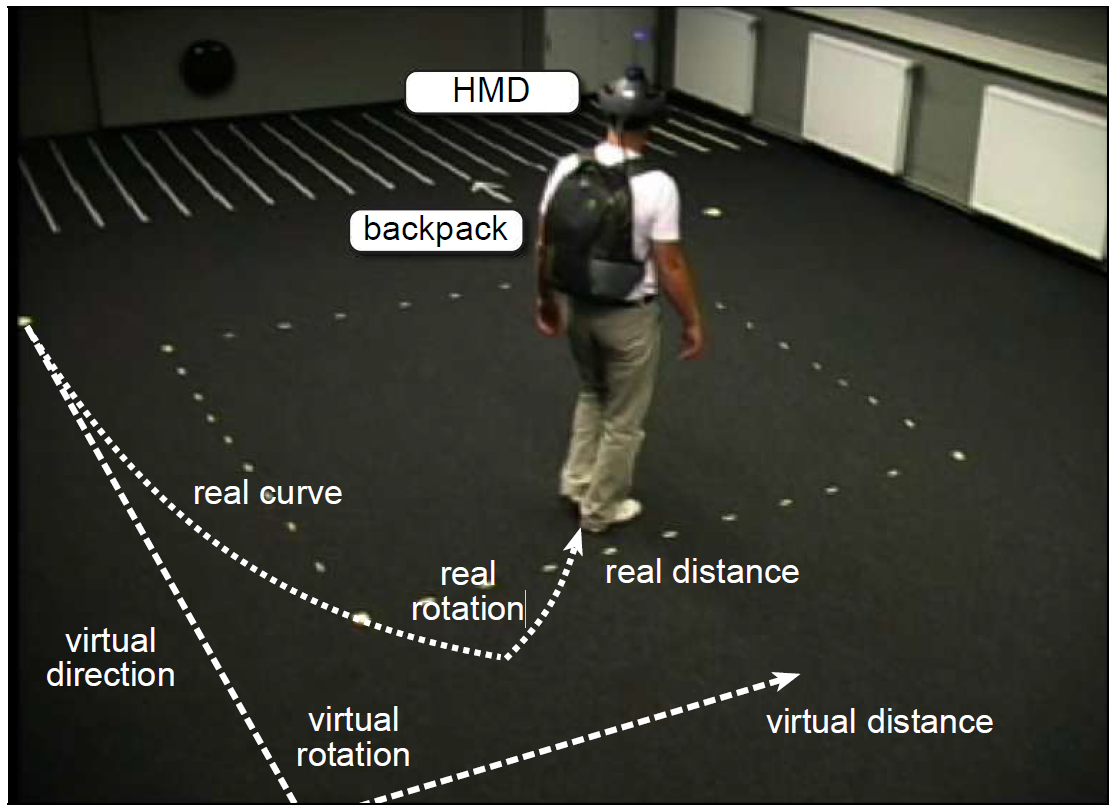
\includegraphics[width=\linewidth]{sections/finalreport/images/steinicke-1.png}	
	\caption{The actual experiment of Steinicke}
\end{figure}
Other studies have investigated the effect of real walking versus other ways of moving forward in the virtual world.
A study by Usoh et al. \cite{usoh} has shown that test subjects that walk in the physical world have a higher presence than so called ``flyers".
In this experiment, the flyers moved forward automatically along their head direction.



	%stay to the point ! only that work that relates to your problem/questions
	
	\begin{frame}{Setup}
	\begin{itemize}
		\item Virtual world with a path
		\item Two groups
			\begin{itemize}
				\item Task
				\item Control
			\end{itemize}
		\item Walk through the physical room
		\item Adjust rotational gains
		\item Maintain presence
	\end{itemize}
	\note{
		So, let's get to the experiment that we designed.
		We're keeping as close as possible to the paper we're trying to reproduce of course, while staying within possible.
		
		There's two test group: One that just walks along the path normally, and one that gets some task while doing this, to see if that distracts them from noticing the gains.
		This task can be anything: We were initially thinking about having people count symbols on the walls or having a light that changes color.
		Ultimately, we settled on math problems.
		
		Presence is very important because people need to be really into the world.
		If we can keep the people present in the world, they will not notice it.
		Break the immersiveness.
	}
\end{frame}

\begin{frame}{Challenges}
	\begin{itemize}
		\item Positional tracking
			\begin{itemize}
				\item Bluetooth triangulating
				\item Oculus DK2 positional tracker
			\end{itemize}
		\item Broken Oculus
		\item 2 hours in the lab per week
	\end{itemize}
	\note{
		We've had some problems- ehrm, faced some challenges of course, during implementation.
		
		First off, positional tracking.
		Change world, need to know where they are.
		Bluetooth, Android, XY, slow.
		Luckily, lab DK2, pos tracker.
		Not really.
		Very small res.
		
		Add to that 2 hours blah.
	}
\end{frame}

\begin{frame}{Solutions}
	\only<1>{
		\begin{itemize}
			\item Gamepad \note{
				We gave up on doing real positional tracking, but we tried to keep it as real as possible by only allowing forward motion.
				This means that while people walked using the controller, they did have to rotate their bodies to change direcion.
			}
		\end{itemize}
	}
	\only<2>{
		\begin{columns}
			\column{0.38\linewidth}
				\centering
				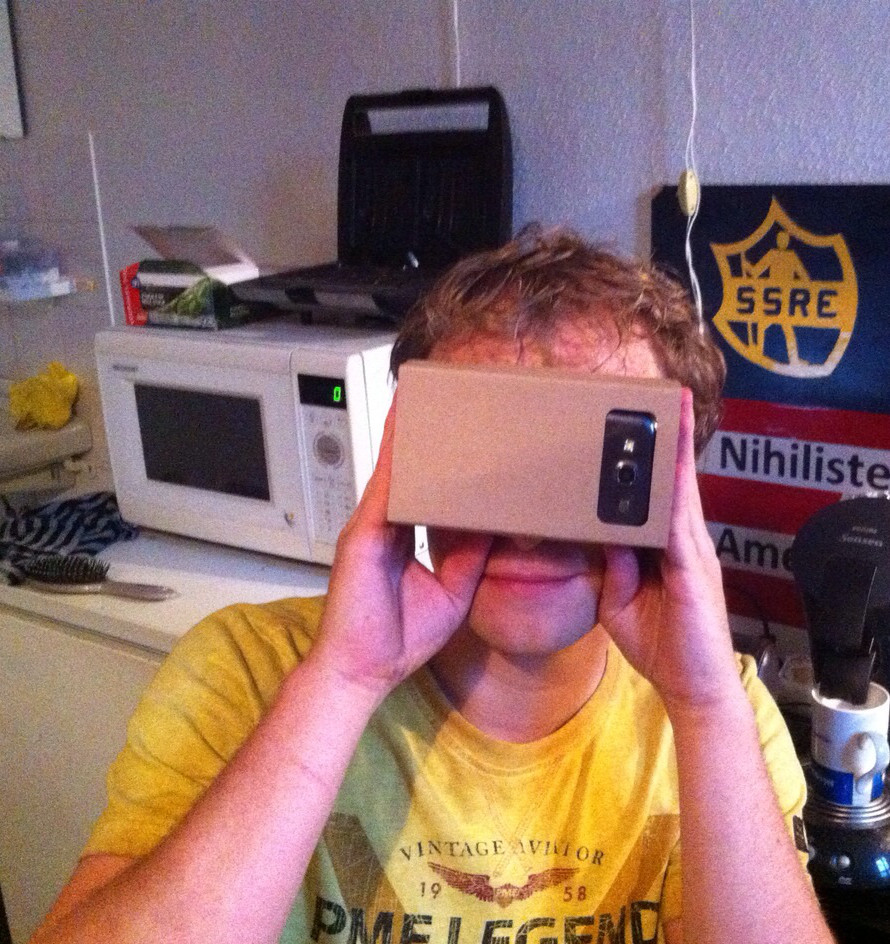
\includegraphics[width=\textwidth]{cardboard}
			\column{0.58\linewidth}
				\begin{itemize}
					\item Gamepad
					\item Google Cardboard (knock-off)
				\end{itemize}
		\end{columns}
	}
\end{frame}

\begin{frame}{Implementation}
	\begin{itemize}
		\item Oculus C++ SDK
		\item Rotational gains
			\begin{itemize}
				\item Change tracking code \note{This happens inside the SDK so not an option\\}
				\item Recalibrate Oculus \note{Not practical because you can't switch easily\\}
				\item Change FPS to influence rotation
				\item Interpret head rotation as extra mouse rotation \note{Weird jump between max and min value, this was noticable for negative gains\\}
			\end{itemize}
		\item Based on \emph{Tinyroom} SDK example
	\end{itemize}
\end{frame}


\begin{frame}{Implementation}
	\begin{figure}
		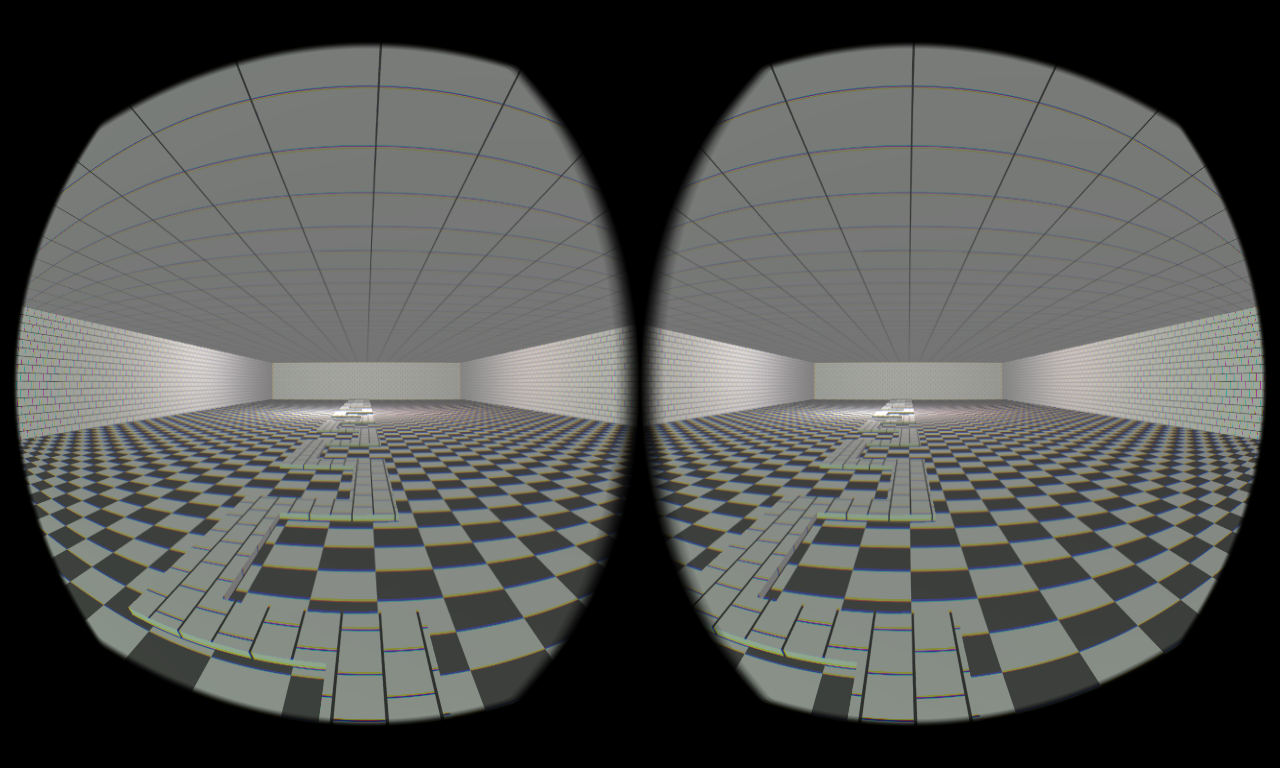
\includegraphics[height=0.8\textheight]{tinyroom}
	\end{figure}
\end{frame}

\begin{frame}{Execution}
	\begin{itemize}
		\item Metaforum
		\item Late at night \note{Because Fontys\\}
		\item Not hard to find subjects \note{Everyone was really excited\\}
		\item But, resetting and calibrating took a long time \note{Because of the jumps\\}
		\item 19 subjects
	\end{itemize}
\end{frame}

\begin{frame}{Execution}
	\begin{figure}
		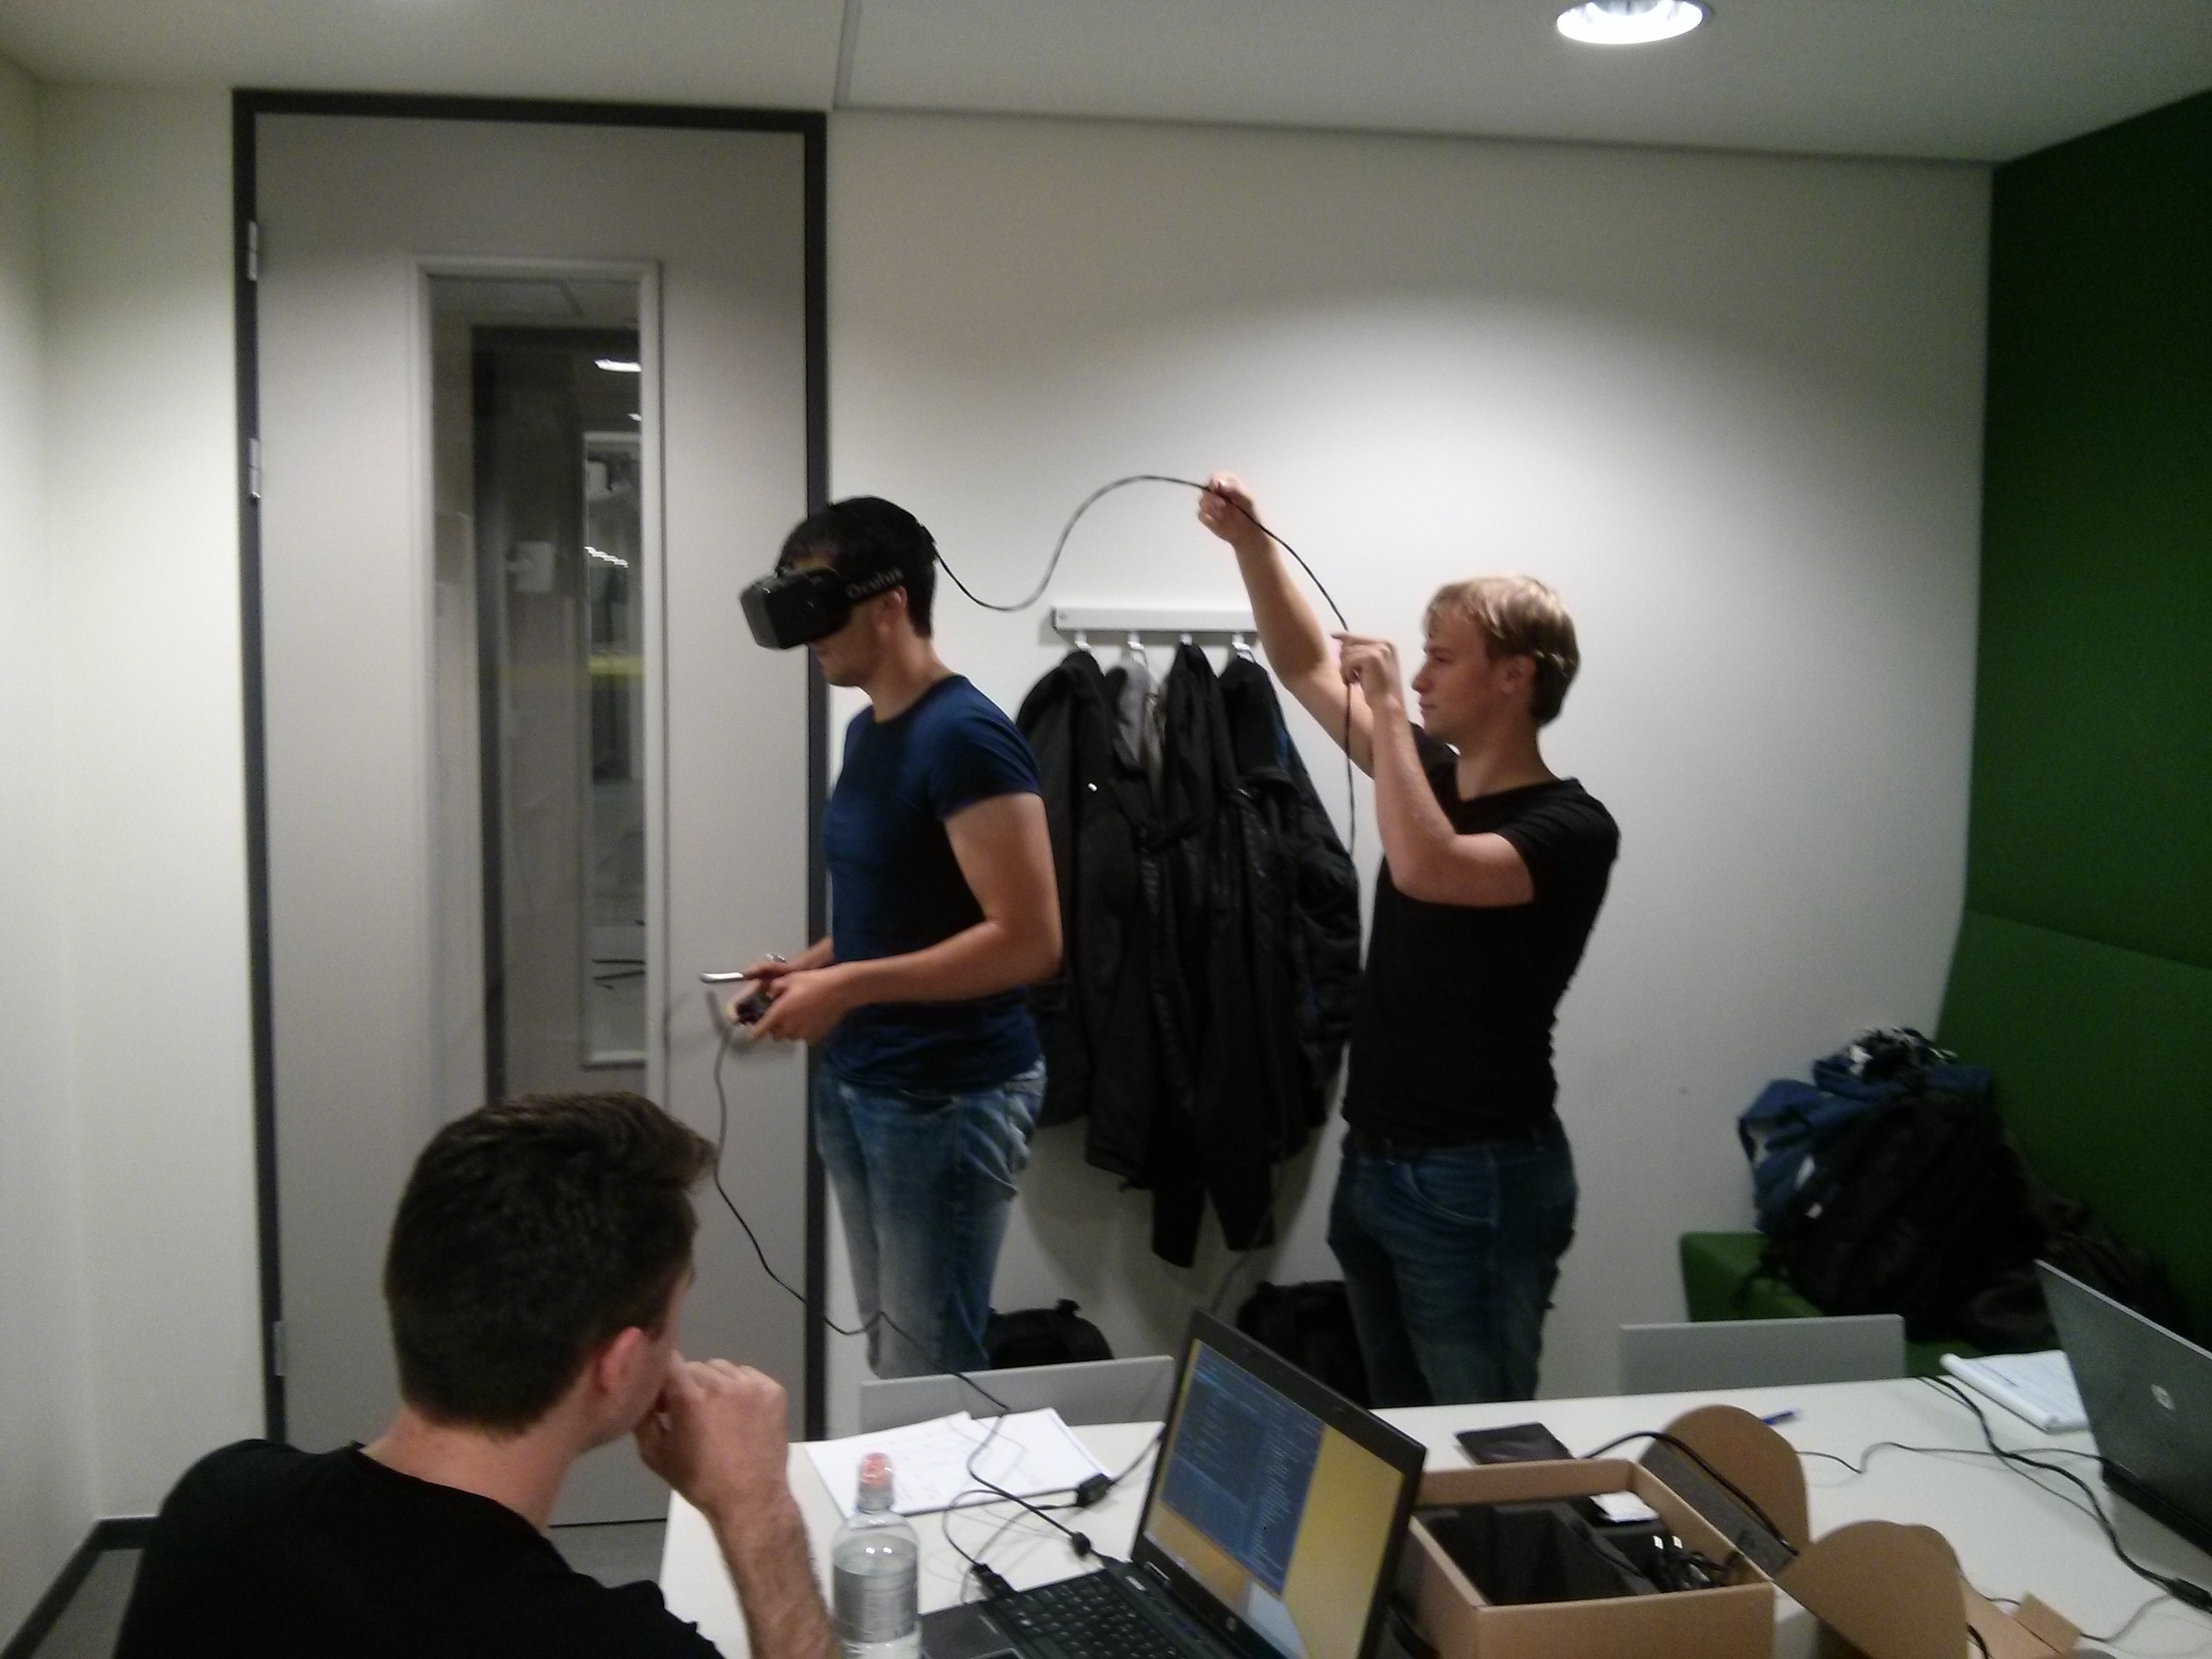
\includegraphics[height=0.8\textheight]{experiment}
	\end{figure}
	\note{Explain how we explained the experiment to the subjects, and what we asked:
		\begin{itemize}
			\item Gain
			\item Gender
			\item Calculation
			\item Notes on condition
		\end{itemize}
	}
\end{frame}


	%Experiment:
	%–detailed description of experiment
	%	• what is the user task / conditions ?
	%	• what is the procedure ? (< 15 min per user !)
	%–discuss relation “research question” <--> “experiment”
	%	• which assumptions are you making ?
	%	• how “complete” is the experiment ?
	%	• what is missing ?
	%– software implementation
	%	• what have you done? indication of how much work was needed?
	
	\subsection{Results}
Now that we have redefined our experiment we discuss the results.
The goal of the experiment is to investigate at what rotational gains the test subjects notice that the virtual world and the real world differ.
Secondly, we are interested in knowing whether this outcome is different when test subjects are engaged in a task (which we have redefined to be simple arithmetic).\\

Now if we look at the results in table 1 we see a couple of columns.
The first column denotes the test subject (or the number of the test).
The second column represents the rotational gain in our implementation, this number is different from the gain as defined by Walker \cite{jwalker}.
Here, 0 means a 1-to-1 mapping from real world to virtual world rotation.
A negative value represents the factor with which virtual world rotation is less than the real world rotation.
Similarly, the positive value represents the factor with which the virtual world rotation is more than the real world rotation.

The third column of table 1 indicates whether or not the test subject did simple arithmetic calculations during the experiment.
Column 4 denotes the test subjects'  response to the following question: ``Did you think your rotation in the virtual world was less, equal or more than your rotation in the real world?"
A ``less" in this column is a correct observation if the gain is negative.
In column 5 the gender of the test subject is shown, we do not conclude anything based on this metric.
In the last column you can see if there are any remarks for the experiment.\\
\\
The first thing that stands out from the results, is that a lot of subjects reported to feeling dizzy or nauseous after the experiment.
Two people felt nauseous, three people felt dizzy and 1 person got a headache doing this experiment.
However, this seems to happen over the entire spectrum of gains tested.
Even though some people seem to be more prone to feeling nauseous from using the Oculus rift then others, having a negative gain (i.e. having to turn further in the real world to achieve a certain rotation in the virtual world) seems to intensify this sensation.
In fact, a test subject opted to stop the experiment due to being very uncomfortable wearing the headset with a negative gain.
This shows us that the human mind might in fact be influenced by the gain.

Especially on the negative gains people felt a little bit sick after (or even during) the experiment.
Even though this is not incorporated in the results we tried the Oculus ourselves with negative gains of up to -0,5 and half of our group got nauseous as well, so when you make the gain too small this has a very negative effect on the body (though we cannot say this for sure since we do not have a lot of tests which confirm this statement).
A possible explanation for this is (including the cases with the positive gain) that people wear the Oculus for the first time in their lives and they have not worn anything like this in their life before.
For a lot of people this technique is really new to them and when you put on the headset a lot of people first have to get used to the Oculus. 
It is not uncommon for some people to have more trouble adjusting to the Oculus than others (especially having different gains).
This could explain the nausea and the dizziness.
People becoming slightly dizzy to the point of feeling nauseous is actually a side effect of the Oculus that has been reported in the media as well.
We also think that the people who wear the Oculus  for the first time are less likely to notice diffrences in the gain, because people who did wear it before can compare the experiment with their previous experience which most likely had no differences in the gains. 

Considering the rotational gain, 3 out of 8 (37.5\%) test subjects correctly noticed a negative gain, 4 out of 8 (50\%) did not notice anything and 1 (12.5\%) even reported a positive gain.
Of the 9 test subjects that experimented with a positive gain, 2 (22.2\%) correctly noticed this, while 6 (66.7\%) did not notice and 1 (11.1\%) even reported a negative gain.
More experiments need to be done to obtain statistically significant results.
From the face of these results, we could say that the negative gain is noticed more often, this is in accordance with our expectations.
We think the people reporting inverse results should be considered outliers.

Another interesting fact is that a lot of people had no notion of what was happening in the virtual world compared to the real world.
In fact it looked the same for a lot of people.
Both the experiment of Walker \cite{jwalker} and ours take place in an empty virtual room with just a path.
It might be interesting to see if the room having additional objects has another effect on the perception of the test subjects
An interesting area for future research is to investigate how the results would differ if the virtual space had more noise, such as buildings or trees around.
Then when a person turns it he or she may notice faster that there is something 'wrong'  with the virtual world.

When we look at the results we see that the group without the tasks 2 out of 9 (22.2\%) noticed the differences in the gain, so 3 out of 9 (30\%)  test subjectives got it correctly.  The group with the task noticed differences in the gain in 6 out of 10 (60\%) times and got it correctly in 3 out of 10 (30\%) times. What is really strange is that the test subjectives of 0.5 and -0.5 noticed completely opposite gains as excepted. The test group without task had 3 out of 9 (30\%) people that felt nauseous or dizzy and the group with task had 4 out of 10 (40\%) people that got nauseous or dizzy. So with a quick glance at the results, we can only mention that there are no significant differences between the test groups, when we compare the correctly noticed differences in the gains and the people that felt dizzy. There is however a big difference between that noticed a difference in the gain, but we do not know for sure if there is a logical explanation or that it is just noise.
\subsection{Comparison to related work}
From our limited test-set, we can not deduce exact negative and positive gains from which the subjects start to notice that the virtual world is different from the real world.
Our result that negative gains are noticed more is in accordance to the study by Walker \cite{jwalker}.
For the possible application of letting people walk around in a large virtual world, but a small physical world, the positive gains are more important and so it is a desirable result that the effects of positive gains are less noticed.
\label{sec:results}
	%results

	\section{Discussion}
We have tried to verify research on the topic of redirected walking.
In particular, we were interested in detecting rotational gains for which participants do no longer feel present.

\subsection{Comparison to related work}
From our limited test-set, we can not deduce exact negative and positive gains from which the subjects start to notice that the virtual world is different from the real world.
Our result that negative gains are noticed more is in accordance to the studies by Steinicke et al. \cite{steinicke1}\cite{steinicke2}
For the possible application of letting people walk around in a large virtual world, but a small physical world, the positive gains are more important and so it is a desirable result that the effects of positive gains are less noticed.\\

Our approach included a different way of moving through the virtual world than physical walking.
We let the test subjects move forward by using a Playstation 3 controller.
This way is comparable to the method of ``flying'' as described by Usoh et al.\cite{usoh}
They have reported higher presence amongst test subjects that walk in the real world while performing the experiment.
This difference could have had an effect on the data from our experiment.
	%show what you have learned, show how this relates to what is known

	\bibliography{bibliography}
	
	\begin{appendix}
	\section{Results table}
\begin{table}
\begin{center}
\begin{tabular}{|c|c|c|c|c|p{4.5cm}|}
\hline
\textbf{Testperson}	&	\textbf{Gain}	&	\textbf{Calculations}	&	\textbf{Rotation}	&	\textbf{Sex}	&	\textbf{Remarks}\\
\hline
1	&	-0.5	&	No	&	Less	&	Female	&	Felt nauseous to the point that she did not finish the experiment\\ \hline
2	&	-0.4	&	No	&	Equal	&	Female	&	Felt a bit dizzy\\ \hline
3	&	-0.3	&	No	&	Equal	&	Male	&	Had a minor headache afterwards, but this could be due to his high blood pressure\\ \hline
4	&	-0.2	&	No	&	Less	&	Female	&	None\\ \hline
5	&	0	&	No	&	Equal	&	Male	&	None\\ \hline
6	&	0.2	&	No	&	Equal	&	Male	&	None\\ \hline
7	&	0.3	&	No	&	Equal	&	Male	&	None\\ \hline
8	&	0.4	&	No	&	Equal	&	Male	&	None\\ \hline
9	&	0.5	&	No	&	Equal	&	Male	&	None\\ \hline
10	&	-0.5	&	Yes	&	More	&	Male	&	Felt nauseous\\ \hline
11	&	-0.3	&	Yes	&	Equal	&	Male	&	None\\ \hline
12	&	-0.2	&	Yes	&	less	&	Male	&	None\\ \hline
13	&	-0.1	&	Yes	&	Equal	&	Male	&	Had consumed a small amount alcohol beforehand\\ \hline
14	&	0	&	Yes	&	More	&	Male	&	Started to feel nauseous, but stated he was prone to feeling nauseous\\ \hline
15	&	0.1	&	Yes	&	More	&	Male	&	Felt dizzy\\ \hline
16	&	0.2	&	Yes	&	Equal	&	Male	&	None\\ \hline
17	&	0.3	&	Yes	&	More	&	Male	&	None\\ \hline
18	&	0.4	&	Yes	&	Equal	&	Male	&	Felt dizzy\\ \hline
19	&	0.5	&	Yes	&	Less	&	Male	&	Had consumed a small amount alcohol beforehand\\ \hline
\end{tabular}
\label{table:results}
\caption{Results of the experiment}
\end{center}
\end{table}\label{Results}
	\section{Tinyroom Implementation}
//TODO include the useful implementation files\label{tinyroom}
	\end{appendix}
\end{document} 
